\documentclass[a4paper,10pt,numbers=noendperiod]{scrartcl}
\setlength\oddsidemargin{0.2cm}
\setlength\evensidemargin{0.2cm}
\setlength\textwidth{15.8cm}

\usepackage{amsfonts}
\usepackage{amssymb}
\usepackage{amsmath}
\usepackage{amsthm}
\usepackage{tikz}
\usepackage{wasysym}
\usepackage{ucs}
\usepackage{stmaryrd}
\usepackage{hyperref}
\usepackage{graphicx}
\usepackage{nicefrac}
\usepackage[english]{babel}
%\usepackage{marvosym}
\usepackage{dsfont}
\usepackage{listings}
\usepackage[utf8x]{inputenc}
\usepackage[T1]{fontenc}
\usepackage{enumitem}
\usepackage{tabularx}
\usepackage{url}
\usepackage{eurosym}

%\def\thesubsubsection{Exercise \arabic{section}.\alph{subsection}.\arabic{subsubsection}} 
%\def\thesubsection{\arabic{section}.\alph{subsection} - } 
%\def\thesection{\arabic{section}}



\lstset{ %
language=XML,                % the language of the code
basicstyle=\footnotesize,       % the size of the fonts that are used for the code
numbers=left,                   % where to put the line-numbers
numberstyle=\footnotesize,      % the size of the fonts that are used for the line-numbers
stepnumber=1,                   % the step between two line-numbers. If it's 1, each line 
numbersep=5pt,                  % how far the line-numbers are from the code
backgroundcolor=\color{white},  % choose the background color. You must add \usepackage{color}
showspaces=false,               % show spaces adding particular underscores
showstringspaces=false,         % underline spaces within strings
showtabs=false,                 % show tabs within strings adding particular underscores
frame=single,                   % adds a frame around the code
tabsize=2,                      % sets default tabsize to 2 spaces
captionpos=b,                   % sets the caption-position to bottom
breaklines=true,                % sets automatic line breaking
breakatwhitespace=false,        % sets if automatic breaks should only happen at whitespace
title=\lstname,                 % show the filename of files included with \lstinputlisting;
}



\author{Ralph Krimmel}
\title{xmpproxy, a proxy server for XMPP}
\subtitle{ Project description and plan }


\begin{document}
\maketitle{}
\thispagestyle{empty}
\newpage
\tableofcontents{}
\newpage
\section{Abstract}
\textit{``The extensible messaging and presence protocol xmpp is an open technology 
for real time communication which powers a wide range of applications including instant messaging, 
presence, multi-party chat, voice and video calls, collaboration, lightweight middleware, 
content syndication and generalized routing of xml data.''}   $_{\tiny http://xmpp.org/about}$ \\

Being widely used in several large communication platforms such as \texttt{Google talk},  % Todo cite
\texttt{XMPP} has become an important protocol for communication via network. This document will describe an 
issue using \texttt{XMPP}'s instant messaging capabilities in a multi client environment and propose a possible solution.
It also contains a time schedule for implementing this solution as a project for the course ``Applied IT project'' at the University 
of Gothenburg.

\section{Introduction}
The \texttt{XMPP} or ``jabber''-protocol supports multiple clients to be connected to the same account at the same time. From the server sides view a connected client is called a \textit{ressource}. The consequence of multiple ressources for the same account is that the server has to decide to which ressource an incoming message, or \textit{stanza} in xmpp terminology, is routed to. This is done via the so called \textit{presence priority} a client can connect with.  The client with the higher priority will receive the message. 
If two or more ressources have the same priority, the server may use some other rule to decide between those or deliver the message to all of them. For example, the server could use the most recent connect time or the most recent activity time. However, the server is not allowed to deliver the stanza to an available resource with a negative priority. %TODO cite 

This behaviour leads to the problem, that conversations and logfiles of conversations may not be complete on every client, if one client connects with a higher priority. Figure \ref{fig:2clients} shows an example where this would be the case. Client A does not know the parts of the conversation that are held from Client B. Also, not just incoming messages will be missing, Client A will not even know about outgoing stanzas from Client B. 
\begin{figure}[h!]
	\begin{center}
		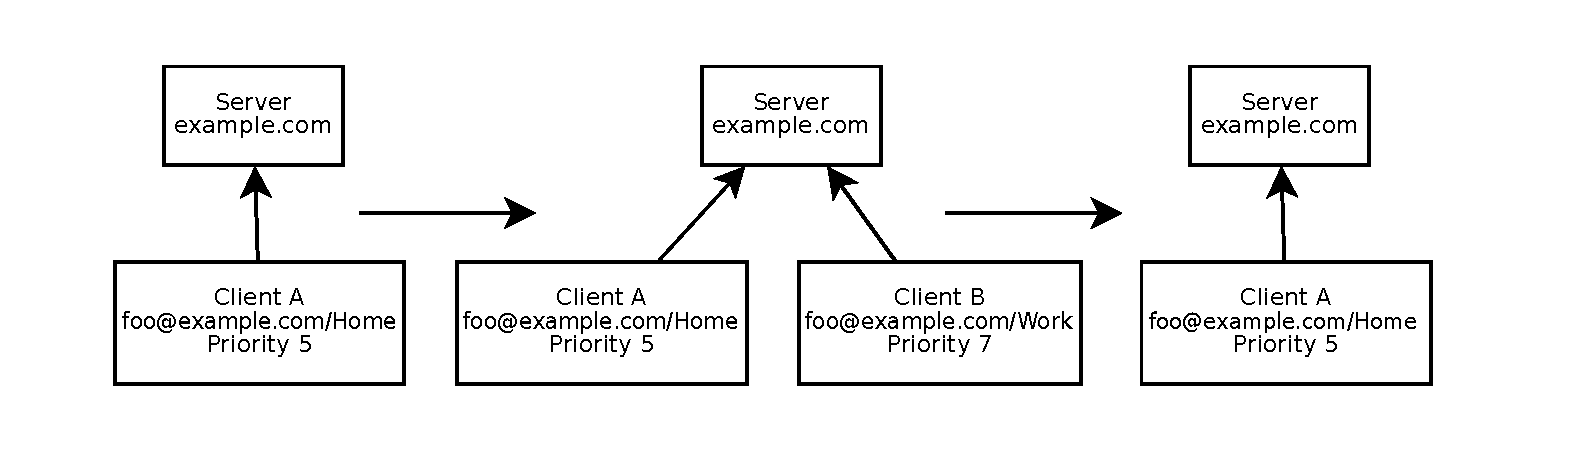
\includegraphics[scale=0.6]{figures/diagram1.pdf}
	\end{center}
	\caption{Clients with 2 different priorities are connected to the same account.}
	\label{fig:2clients}
\end{figure}


A possible solution for this issue may be the use of a proxy server as it can be seen in figure \ref{fig:2clientsproxy}. This server will make sure, that every incoming stanza will reach both clients and every outgoing stanza will be sent to every ressource as well as to the targeted server.

\begin{figure}[h!]
	\begin{center}
		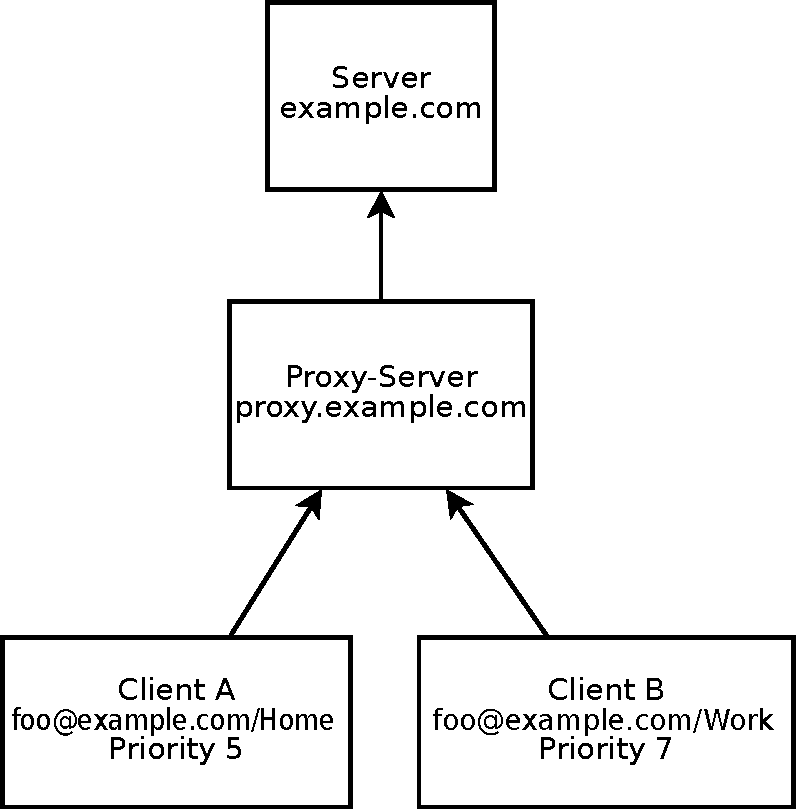
\includegraphics[scale=0.4]{figures/diagram3.pdf}
	\end{center}
	\caption{Two clients connected to a proxy.}
	\label{fig:2clientsproxy}
\end{figure}
\newpage
\section{Technology}
\subsection{Software choice}
For implementing the xmpp proxy server several design descisions had to me made. First of all a programming language was chosen. Possible languages were Perl, C, C++ and Java because of the preferences of the author. The criteria for the programming language was first of all the availability of proper libraries that deal with the xmpp protocol, both server and client side.  Unfortunately, this excluded all languages except perl because there are just few xmpp server libraries at all. Therefore the xmpp proxy server will make use of the \texttt{djabberd} xmpp/jabber server although it lacks a proper documentation.
\subsection{Djabberd}
Djabberd is a modular, scalable and extensible jabber server written in perl where almost everything defers to hooks to be implemented by plugins. %cite
It is written and maintained by \textit{Brad Fitzpatrick}, \textit{Artur Bergman} and \textit{Jonathan Steinert}.
When this document was created, the most recent version of djabberd was 0.85, released on the thirteenth of June in 2011. Having a modular structure, djabberd is a perfect framework for building the required proxy server because it offers hooks for modifying the behaviour of the authentication and authorization process, roster storage and message delivery. Also, \texttt{djabberd} can be used in environments which require a high performance for it is asynchrone/event-based, using epoll on linux 2.6.
\subsection{xmpproxy}
\subsubsection{Configuration}
The configuration of \texttt{xmpproxy} is done via a single xml configuration file. The file, \texttt{proxy.xml}, can be found in the same directory as the \texttt{xmpproxy} executable. The file stores all the non-ephemeral information of the user database (names, passwords, options) and \texttt{xmpproxy} specific options like the node name of the server. 
Here is an example configuration file:
\begin{lstlisting}
<config>
	<node name="fluttershy"></node>

	<user name="test" passwd="bar" resource="access">
		<account jid="test@milk-and-cookies.net" passwd="test" resource="xmpproxy"/>
		<account jid="bla@milk-and-cookies.net" passwd="bla" resource="xmpproxy"/>
	</user>
</config>
\end{lstlisting}
\textbf{Cave}: The syntax of this file may change in future versions of \texttt{xmpproxy}.


\subsubsection{Logging}
	\texttt{xmpproxy} uses \texttt{log4perl} to create nice looking, configurable log files. It offers five different log levels (ordered from the most to the least verbose):
	\begin{itemize}
		\item DEBUG
		\item INFO
		\item WARN
		\item ERROR
		\item CRITICAL
	\end{itemize}
	The desired loglevel can be adjusted by setting the environmental variable ``LOGLEVEL'' to the wanted value, e.g.\\ \texttt{\$ export LOGLEVEL=DEBUG}
		

\subsubsection{Modules}
This is just a short description of the available modules. For a full API documentation see \textit{refman.pdf}
	\paragraph{xmpproxy::Userdb and xmpproxy::User} 
	Those are classes for the management of users in xmpproxy. A \texttt{xmpproxy::Userdb} object stores instances of User objects. It also offers methods to add, delete and modify users. A \texttt{xmpproxy::User} object holds information of a user. That information is username, password and a list of \texttt{DJabberd::Queue::ClientOut} objects, which represent a client connection.
	\paragraph{DJabberd::Authen::Proxy}
	Module that queries the xmpp user database and checks the provided credentials.
	\paragraph{Djabberd::Connection::ClientOut and DJabberd::Queue::ClientOut}
	Those two classes are needed to make DJabberd connecting to another Jabberserver as a client. \texttt{DJabberd::Stanza::SASL} is used if SASL authentication is supported. 
	\paragraph{DJabberd::RosterStorage::Proxy}
	Module for roster (``buddylist``) managment. Has methods to fetch and modify the rosters for each proxy account. Currently just basic functions for getting rosters.
	\paragraph{DJabberd::Delivery::Local}
	The task of this module is to deliver incoming message/presence stanzas properly. To do this, the ''to``-attribute has to be rewritten to deliver the message to \texttt{xmpproxy} users.
	\paragraph{DJabberd::Delivery::Proxy}
	Module for delivering all outgoing message/presence stanzas.(Partly) implements XEP-0280(Message carbons). This means that it mirrors all outgoing message stanzas to each connected client. Also, for forwarding purposes, the ''from`` attribute is rewritten.
	\paragraph{DJabberd::IQ}
	Module that handles all IQ stanzas. Client side functions have been added.
	\paragraph{DJabberd::Message}
	Module that handles all message stanzas. Client side functions have been added.
	\paragraph{DJabberd::Presence}
	Module that handles all presence stanzas. Client side functions have been added.
%\subsection{Net::XMPP}
%\texttt{Net::XMPP} is a perl package that provides access to XMPP client side functions for the perl programming language. It is maintaned by \textit{Eric Hacker} and versioned 1.02 at the time this document was written.
%It can be utilized using its object oriented interface. 
%There are objects available which hold the actual client functions like login, wait for messages, send messages and logout. 
%Also there are objects for storing and handling Jabber IDs (\texttt{Net::XMPP::JID}), messages (\texttt{Net::XMPP::Message}), presence information (\texttt{Net::XMPP::Presence}) and Info/Query namespaces (\texttt{Net::XMPP::IQ}).  
\newpage
\section{Tasks}
The following tasks are to be completed:
\begin{itemize}
	\item Studies of literature and source code
	\item Userdatase \texttt{xmpproxy::Userdb} and \texttt{xmpproxy::User}
	\item Module for proxy authentication \texttt{DJabberd::Authen::Proxy}
	\item Basic XMPP client functionalities \texttt{DJabberd::Connection::ClientOut}, \texttt{DJabberd::Queue::ClientOut} and \texttt{DJabberd::Stanza::SASL}
	\item Module for proxy roster handling \texttt{DJabberd::RosterStorage::Proxy}
	\item Module for proxy presence handling \texttt{DJabberd::Presence} and \texttt{DJabberd::Delivery::Proxy}
	\item Module for message delivery \texttt{DJabberd::Message} and \texttt{DJabberd::Delivery::Proxy}
	\item Module for basic IQ handling \texttt{DJabberd::IQ}
	\item (Optional) Module for proxy groupchat 
	\item (Optional) Module for proxy jingle (Voice/Video via jabber)	
	\item (Optional) root admin bot                                  
	\item Write Documentation	
	\item Write Report
	\item Create presentation
\end{itemize}

\newpage
\section{Schedule}
The \texttt{xmpproxy} software will be written in the context of the course ``Applied IT Project'' course at the University of Gothenburg. This requires to ``formulate and execute a finite Applied IT project within a limited time-frame''. 
Therefore it is neccessary to schedule the tasks described in the previous sections. 
Table \ref{tab:estimatedtime} shows the the estimated time every task will take. The minimum required amount of time this project will need is 200 hours. Due to the size of the project, the time plan will cover 280 hours of work. Those 300 hours are distributed over 18 weeks. Four of those 18 weeks won't be available for activity because of exam preparation and as backup time in case of unforseen consequences (illness, design mistakes) or implementation difficulties. The project is beeing executed mid semester while one other 7.5 ECTS course is absolved. That means that 50\% of the effort can be put into \texttt{xmpproxy}. Therefore, the average weekly time used for working on \texttt{xmpproxy} is approximately 20h.


\begin{table}[h]
	\centering
	\begin{tabularx}{\textwidth}{|l|X|c|}
	\hline
	\textbf{Date (11/12)} & \textbf{Task} & \textbf{Time (in h)} \\
	\hline
	\hline
	 1.10. - 7.10. & Studies of literature & 20 \\
	\hline
         8.10. - 14.10. & Project plan & 20 \\
	\hline
	15.10. - 21.10. & First exam period & - \\
        \hline
	22.10. - 25.10. & User database & 10 \\
	\hline
	26.10. - 29.10. & Module for proxy authentication & 10 \\
	\hline
	30.10. - 13.11. & Basic XMPP client functionalities  & 40 \\ 
	\hline
	14.11. - 20.11. & Module for proxy roster handling & 20 \\ 
	\hline
	21.11. - 27.11. & Module for proxy presence handling & 20 \\ 
	\hline
	28.11. -  3.12. & Module for message delivery & 20 \\
	\hline
	 4.11. -  9.11  & Module for basic IQ handling & 20 \\
	\hline
	10.12. - 16.12. & Second exam period & - \\
	\hline
	17.12  - 22.12  & Module for basic IQ handling & 20 \\ 
	\hline
	23.12  -  3.12  & Documentation,Report,Praesentation & 80 \\ 
	\hline
	  4.1  -   9.1  & Backup time & - \\
	\hline
	       -        & (Optional) Module for proxy groupchat & ? \\
	\hline
	       -        & (Optional) Module for proxy jingle (Voice/Video via jabber)  & ? \\
	\hline
	       -        & (Optional) root admin bot                                    & ? \\ 
	\hline
	\end{tabularx}
	\caption{Time plan}
	\label{tab:estimatedtime}
\end{table}

\newpage
\section{Literature}
\begin{itemize}
	\item \texttt{Programming jabber - extending XML messaging} by DJ Adams\\
	\item \url{http://xmpp.org/rfcs/rfc6120.html}\\
	\item \url{http://xmpp.org/rfcs/rfc6121.html}\\
	\item \url{http://xmpp.org/rfcs/rfc6122.html}\\
	\item \url{http://search.cpan.org/~mart/DJabberd-0.85/}\\
	\item All the DJabberd sources
\end{itemize}


\end{document} 
